\begin{examnotes}{Exam 1 Notes}
    \subsubsection*{Data Frames}

    A data frame in Pandas is a two-dimensional, size-mutable, and potentially heterogeneous tabular data structure with labeled axes (rows and columns). It's akin to a spreadsheet or SQL table and 
    is one of the most commonly used Pandas data structures.

    You can create a data frame from various sources, such as:

    \begin{itemize}
        \item Lists
        \item Dictionaries
        \item NumPy arrays
        \item CSV files
        \item SQL databases
    \end{itemize}

    The structure of data frames can be summed up by:

    \begin{itemize}
        \item \textbf{Rows}: Each row represents a single observation or record.
        \item \textbf{Columns}: Each column represents a variable or feature. Columns can be of different data types (integer, string, float, etc.).
        \item \textbf{Index}: This is the `key' for rows, similar to an index in a database. It’s an immutable array, allowing fast access to data.
    \end{itemize}

    Some operations that can be used with data frames are:

    \begin{itemize}
        \item \textbf{Data Manipulation}: Adding, deleting, and modifying both rows and columns.
        \item \textbf{Filtering}: Selecting a subset of rows or columns based on some criteria.
        \item \textbf{Sorting and Grouping}: Organizing data based on values in certain columns.
        \item \textbf{Merging and Joining}: Combining multiple data frames.
        \item \textbf{Handling Missing Data}: Identifying and imputing missing values.
    \end{itemize}

    \begin{highlight}[Data Frame Operation Examples]
        Here are some examples of data frame manipulation in pandas:

        \subsubsection*{Creation}

    \begin{code}[Python]
    import pandas as pd

    # Creating a data frame from a dictionary
    data = {'Name': ['Alice', 'Bob', 'Charlie'], 
            'Age': [25, 30, 35],
            'City': ['New York', 'Los Angeles', 'Chicago']}
    df = pd.DataFrame(data)            
    \end{code}

        \subsubsection*{Adding A Column}

    \begin{code}[Python]
    # Adding a new column
    df['Salary'] = [70000, 80000, 90000]        
    \end{code}

        \subsubsection*{Deleting A Column}

    \begin{code}[Python]
    # Deleting a column
    df.drop('Age', axis=1, inplace=True)        
    \end{code}

        \subsubsection*{Filtering Data}

    \begin{code}[Python]
    # Filtering rows where Salary is greater than 75000
    high_earners = df[df['Salary'] > 75000]        
    \end{code}

        \subsubsection*{Sorting Data}

    \begin{code}[Python]
    # Sorting data by Salary in descending order
    df_sorted = df.sort_values(by='Salary', ascending=False)        
    \end{code}

        \subsubsection*{Merging Data Frames}

    \begin{code}[Python]
    # Creating another data frame
    additional_data = pd.DataFrame({'Name': ['Alice', 'Bob'], 'Experience': [5, 10]})
    
    # Merging data frames
    merged_df = pd.merge(df, additional_data, on='Name', how='left')        
    \end{code}

        \subsubsection*{Handling Missing Data}

    \begin{code}[Python]
    # Filling missing values with zero
    df_filled = df.fillna(0)        
    \end{code}

        \subsubsection*{Reading Data}

    \begin{code}[Python]
    # Reading data from a CSV file
    df_from_csv = pd.read_csv('data.csv')
    
    # Writing data to a CSV file
    df.to_csv('output.csv', index=False)        
    \end{code}
    \end{highlight}

    \subsubsection*{Combinatorics}

    Combinatorics is a branch of mathematics dealing with the study of countable, discrete structures and their properties. It's particularly important in computer science, where understanding how to 
    count and arrange objects is crucial for algorithm design, data structure optimization, and problem-solving. Here's a summary of the key concepts in combinatorics:

    \begin{itemize}
        \item \textbf{Counting Principles}
        \begin{itemize}
            \item \textbf{The Rule of Sum}: If there are $A$ ways to do something and $B$ ways to do another thing, and these two things cannot happen at the same time, then there are $A + B$ ways 
            to choose one of these actions.
            \item \textbf{The Rule of Product}: If there are $A$ ways to do something and $B$ ways to do another thing after that, then there are $A \cdot B$ ways to perform both actions.
        \end{itemize}
        \item \textbf{Permutations}
        \begin{itemize}
            \item Permutations are the arrangements of objects in a specific order.
            \item The number of permutations of $n$ distinct objects is $n!$ ($n$ factorial), which is the product of all positive integers up to $n$.
            \item For arranging $r$ objects out of $n$ available objects, the formula is
            \begin{center}
                \begin{highlightbox}
                    ^{n}P_{r} = \frac{n!}{(n - r)!}.
                \end{highlightbox}
            \end{center}
        \end{itemize}
        \item \textbf{Combinations}
        \begin{itemize}
            \item Combinations refer to the selection of objects without regard to the order.
            \item The number of ways to choose $r$ objects from $n$ different objects is given by 
            \begin{center}
                \begin{highlightbox}
                    {n \choose r} = \frac{n!}{r!(n - r)!}.
                \end{highlightbox}
            \end{center}
            \item Combinations are used when the order doesn't matter.
        \end{itemize}
        \item \textbf{Binomial Theorem}
        \begin{itemize}
            \item It provides a formula for the expansion of powers of a binomial (sum of two terms).
            \item The Binomial Theorem states that:
            \begin{center}
                \begin{highlightbox}
                    (a + b)^{n} = \sum_{k = 0}^{n} {n \choose k} \cdot a^{n - k} \cdot b^{k}
                \end{highlightbox}
            \end{center}
            \begin{itemize}
                \item This means the expansion is a sum of terms, where the exponents of a start at $n$ and decrease to 0, while the exponents of $b$ start at 0 and increase to $n$. The coefficients 
                of each term are the corresponding binomial coefficients.
            \end{itemize}
            \item The coefficients of the terms in the expansion are the binomial coefficients, which can be calculated using combinations.
        \end{itemize}
        \item \textbf{Binomial Distribution}
        \begin{itemize}
            \item A binomial distribution is a discrete probability distribution that models the number of successes in a fixed number of independent Bernoulli trials. A Bernoulli trial is an experiment 
            with exactly two possible outcomes, typically termed "success" and "failure".
            \item In the context of the binomial distribution, $P(x = k)$ denotes the probability of getting exactly $k$ successes in $n$ trials. The formula for this is
            \begin{center}
                \begin{highlightbox}
                    P(x = k) = {n \choose k} \cdot p^{k} \cdot (1 - p)^{n - k}.
                \end{highlightbox}
            \end{center}
            \begin{itemize}
                \item $\binom{n}{k}$ (read as "$n$ choose $k$") is the binomial coefficient, representing the number of ways to choose $k$ successes from $n$ trials.
                \item $p$ is the probability of success on an individual trial.
                \item $1 - p$ is the probability of failure (since the trials are binary, the sum of the probabilities of success and failure is 1).
                \item $p^{k}$ is the probability of having $k$ successes.
                \item $(1 - p)^{n - k}$ is the probability of having $n - k$ failures.
            \end{itemize}
        \end{itemize}
    \end{itemize}

    \subsubsection*{groupby}

    The \texttt{groupby} method is used to split data into groups based on some criteria, apply a function to each group independently, and then combine the results into a data structure. The process 
    is often summarized as split-apply-combine.

    The way \texttt{groupby} works is by the following:

    \begin{itemize}
        \item \textbf{Split}: The data is divided into groups based on one or more keys. This is done by mapping a function over the index or columns of the DataFrame.
        \item \textbf{Apply}: A function is applied to each group independently. This function could be an aggregation (computing a summary statistic), transformation (standardizing data within a group), 
        or filtration (removing data based on group properties).
        \item \textbf{Combine}: The results of the function application are combined into a new data structure.
    \end{itemize}

    The basic syntax for how \texttt{groupby} works is as follows:

    \begin{code}[Python]
    df.groupby(by=None, axis=0, level=None, as_index=True, sort=True, group_keys=True, squeeze=NoDefault.no_default, observed=False, dropna=True)
    \end{code}

    \begin{itemize}
        \item \textbf{by}: Specifies the grouping criteria. Can be a function, column name, or list of column names.
        \item \textbf{axis}: Determines whether to group by rows (0) or columns (1).
        \item \textbf{level}: If the axis is a MultiIndex (hierarchical), groups by a particular level or levels.
        \item \textbf{as\_index}: For aggregated output, returns object with group labels as the index. Setting it to False will return group labels in the columns.
        \item \textbf{sort}: Sorts group keys. By default, it's set to True.
    \end{itemize}

    \begin{highlight}[groupby Example]
        Here is a simple example of utilizing \texttt{groupby} in Pandas:

    \begin{code}[Python]
    import pandas as pd

    # Example DataFrame
    data = {
        'Date': ['2023-01-01', '2023-01-01', '2023-01-02', '2023-01-02', '2023-01-03'],
        'Product': ['A', 'B', 'A', 'A', 'B'],
        'Sales': [100, 200, 150, 100, 250]
    }
    df = pd.DataFrame(data)
    
    # Group by 'Product' and sum up the sales
    grouped_df = df.groupby('Product')['Sales'].sum()
    
    print(grouped_df)            
    \end{code}
    \end{highlight}

    \subsubsection*{agg}

    The \texttt{agg} method in Pandas, when used with groupby, is a versatile tool for performing multiple aggregation operations on your grouped data. It allows for more flexibility than just applying 
    a single aggregate function like \texttt{sum} or \texttt{mean} directly. With \texttt{agg}, you can apply different aggregation functions to your data simultaneously, and even specify custom functions 
    to suit your analysis needs.

    After grouping your DataFrame with the \texttt{groupby} method, you can use \texttt{agg} to specify one or more aggregation operations to apply to the grouped data. \texttt{agg} can take a variety 
    of inputs:

    \begin{itemize}
        \item A single aggregation function as a string (e.g. \texttt{'sum'}, \texttt{'mean'}).
        \item A list of functions (e.g., \texttt{['sum', 'mean', 'max']}), applying each function to each column of each group.
        \item A dictionary where keys are column names and values are functions or lists of functions, allowing different aggregation for different columns.
    \end{itemize}

    \begin{highlight}[agg Example]
        Expanding on the previous example that was used with \texttt{groupby}, the example below encapsulates how to use the \texttt{agg} function with \texttt{groupby}:

    \begin{code}[Python]
    import pandas as pd

    # Example DataFrame
    data = {
        'Date': ['2023-01-01', '2023-01-01', '2023-01-02', '2023-01-02', '2023-01-03'],
        'Product': ['A', 'B', 'A', 'A', 'B'],
        'Sales': [100, 200, 150, 100, 250]
    }
    df = pd.DataFrame(data)
    
    # Group by 'Product' and apply multiple aggregation functions to 'Sales'
    grouped_df = df.groupby('Product')['Sales'].agg(['sum', 'mean', 'max'])
    
    print(grouped_df)        
    \end{code}
    This would output the total, average, and maximum sales for each product.

    More advanced usage can be applied to the \texttt{agg} function, below is an example with the previous data frame in the last example of this advanced usage:

    \begin{code}[Python]
    grouped_df = df.groupby('Product').agg({
        'Sales': ['sum', 'mean'],
        'Date': ['min', 'max']
    })        
    \end{code}
    This performs a sum and mean aggregation on the \texttt{Sales} and finds the minimum and maximum \texttt{Date} for each \texttt{Product}.
    \end{highlight}

    \subsubsection*{Joining DataFrames}

    Joining data frames is a fundamental operation in data analysis, allowing you to combine data from different sources based on common identifiers. Pandas offers several methods for joining DataFrames, 
    akin to SQL joins, including \texttt{merge}, \texttt{join}, and \texttt{concat}. Understanding these methods and when to use each is key to effective data manipulation.

    \begin{enumerate}
        \item \textbf{merge}: The \texttt{merge} function is the most versatile method for joining two DataFrames. It allows you to perform inner, outer, left, and right joins by specifying how you 
        want the DataFrames to be merged.
        \begin{itemize}
            \item \textbf{Syntax}: \scriptsize{\texttt{pd.merge(left, right, how='inner', on=None, left\_on=None, right\_on=None, left\_index=False, right\_index=False)}} \normalsize
            \item \textbf{Parameters}:
            \begin{itemize}
                \item \texttt{left, right}: The DataFrames you want to join.
                \item \texttt{how}: Specifies the type of join \texttt{('left', 'right', 'outer', 'inner')}.
                \item \texttt{on}: The column(s) to join on. Must be found in both DataFrames.
                \item \texttt{left\_on, right\_on}: Columns from the left and right DataFrames to use as keys if they have different names.
                \item \texttt{left\_index, right\_index}: If True, use the index (row labels) from the left or right DataFrame as its join key(s).
            \end{itemize}
        \end{itemize}
        \begin{highlight}[merge Example]
            Below is a simple example of how \texttt{merge} works by joining DataFrames:

    \begin{code}[Python]
    import pandas as pd

    # Example DataFrames
    df1 = pd.DataFrame({'key': ['A', 'B', 'C', 'D'], 'value': range(4)})
    df2 = pd.DataFrame({'key': ['B', 'D', 'D', 'E'], 'value': range(4, 8)})
    
    # Inner join on 'key'
    inner_joined = pd.merge(df1, df2, on='key', how='inner')
    
    # Outer join on 'key'
    outer_joined = pd.merge(df1, df2, on='key', how='outer')            
    \end{code}
        \end{highlight}
        \item \textbf{join}: The \texttt{join} method is a convenient method for combining DataFrames based on their indexes or on a key column. It's a simpler interface than \texttt{merge} for index-based 
        joining.
        \begin{itemize}
            \item \textbf{Syntax}: \texttt{DataFrame.join(other, on=None, how='left', lsuffix='', rsuffix='')}
            \item \textbf{Parameters}:
            \begin{itemize}
                \item \texttt{other}: The DataFrame to join with.
                \item \texttt{on}: The column or index level names to join on in the \texttt{other} DataFrame. Must be found in both the calling DataFrame and \texttt{other}.
                \item \texttt{how}: Type of join \texttt{('left', 'right', 'outer', 'inner')}.
                \item \texttt{lsuffix, rsuffix}: Suffixes to apply to overlapping column names in the DataFrames.
            \end{itemize}
        \end{itemize}
        \begin{highlight}[join Example]
            Below is a simple example of how \texttt{join} works by joining DataFrames:
    \begin{code}[Python]
    # Assuming df1 and df2 from the previous example
    # Join df2 to df1 using the index of df1 and the 'key' column of df2
    joined = df1.join(df2.set_index('key'), on='key', how='left', lsuffix='_df1', rsuffix='_df2')        
    \end{code}
        \end{highlight}
        \item \textbf{concat}: The \texttt{concat} function is used for concatenating DataFrames along a particular axis (row-wise or column-wise). It's useful for stacking DataFrames vertically or horizontally.
        \begin{itemize}
            \item \textbf{Syntax}: \texttt{pd.concat(objs, axis=0, join='outer')}
            \item \textbf{Parameters}:
            \begin{itemize}
                \item \texttt{objs}: A sequence of DataFrames to concatenate.
                \item \texttt{axis}: The axis to concatenate along (0 for rows, 1 for columns).
                \item \texttt{join}: How to handle indexes on other axis \texttt{('outer', 'inner')}.
            \end{itemize}
        \end{itemize}
        \begin{highlight}[concat Example]
            Below is a simple example of how \texttt{concat} works by joining DataFrames:
    \begin{code}[Python]
    # Vertical concatenation
    vertical_concat = pd.concat([df1, df2])
    
    # Horizontal concatenation, assuming same indexes
    horizontal_concat = pd.concat([df1, df2], axis=1)        
    \end{code}
        \end{highlight}
    \end{enumerate}

    \subsubsection*{Measures Of Central Tendency}

    There are core ways we can measure information about data, below are some pertinent ways that we measure central tendency in data science:

    \begin{enumerate}
        \item \textbf{Mean} - The mean, often referred to as the average, is calculated by summing all the values in the data set and then dividing by the number of values. It's a measure that is 
        sensitive to outliers, meaning that a single very high or very low value can significantly affect the mean.

        The formula for calculating the mean of a data set is:

        \begin{center}
            \begin{highlightbox}
                \text{Mean} = \frac{\sum_{i = 1}^{n} x_{i}}{n}
            \end{highlightbox}
        \end{center}
        where $x_{i}$ represents each value in the dat set and $n$ is the total number of values.
        \item \textbf{Median} - The median is the middle value in a data set when the values are arranged in ascending or descending order. If there's an even number of observations, the median is the 
        average of the two middle numbers. Unlike the mean, the median is not affected by outliers, making it a better measure of central tendency for skewed distributions.
        \begin{itemize}
            \item \textbf{Finding The Median}:
            \begin{itemize}
                \item Arrange the data in ascending order.
                \item If the number of observations $(n)$ is odd, the median is the value at position $\frac{n + 1}{2}$.
                \item If $n$ is even, the median is the average of the values at positions $\frac{n}{2}$ and $\frac{n}{2} + 1$.
            \end{itemize}
        \end{itemize}
        \item \textbf{Mode} - The mode is the value that appears most frequently in a data set. A data set may have one mode (unimodal), more than one mode (bimodal or multimodal), or no mode at all 
        if all values occur with the same frequency. The mode is particularly useful for categorical data where we want to identify the most common category.
        \begin{itemize}
            \item \textbf{Key Characteristics}:
            \begin{itemize}
                \item The mode is the only measure of central tendency that can be used with nominal data (data categorized without a natural order).
                \item A data set may have multiple modes, making it a good measure for understanding variability in data.
            \end{itemize}
        \end{itemize}
    \end{enumerate}

    \begin{highlight}[Central Tendency Example]
        Consider the simple data set: \texttt{2,3,3,5,7,10}
        \subsubsection*{Mean}
        \begin{equation*}
            \text{Mean} = \frac{\sum_{i = 1}^{n} x_{i}}{n} = \frac{2 + 3 + 3 + 5 + 7 + 10}{6} = \frac{30}{6} = 5.
        \end{equation*}
        \subsubsection*{Median}
        The data set is even, so the median is the average of the middle values (3rd and 4th values):
        \begin{equation*}
            \text{Median} = \frac{3 + 5}{2} = \frac{8}{2} = 4.
        \end{equation*}
        \subsubsection*{Mode}
        The value \texttt{3} appears most frequently, so the mode of this data set is \texttt{3}.
    \end{highlight}

    \subsubsection*{Plot Interpretation}

    Plots are a vital concept in data science. Interpreting them is a vital skill and important for understanding data and how to draw conclusions. For this, we have created three types of plots that
    are common in data science. These plots can be seen below.

    \begin{center}
        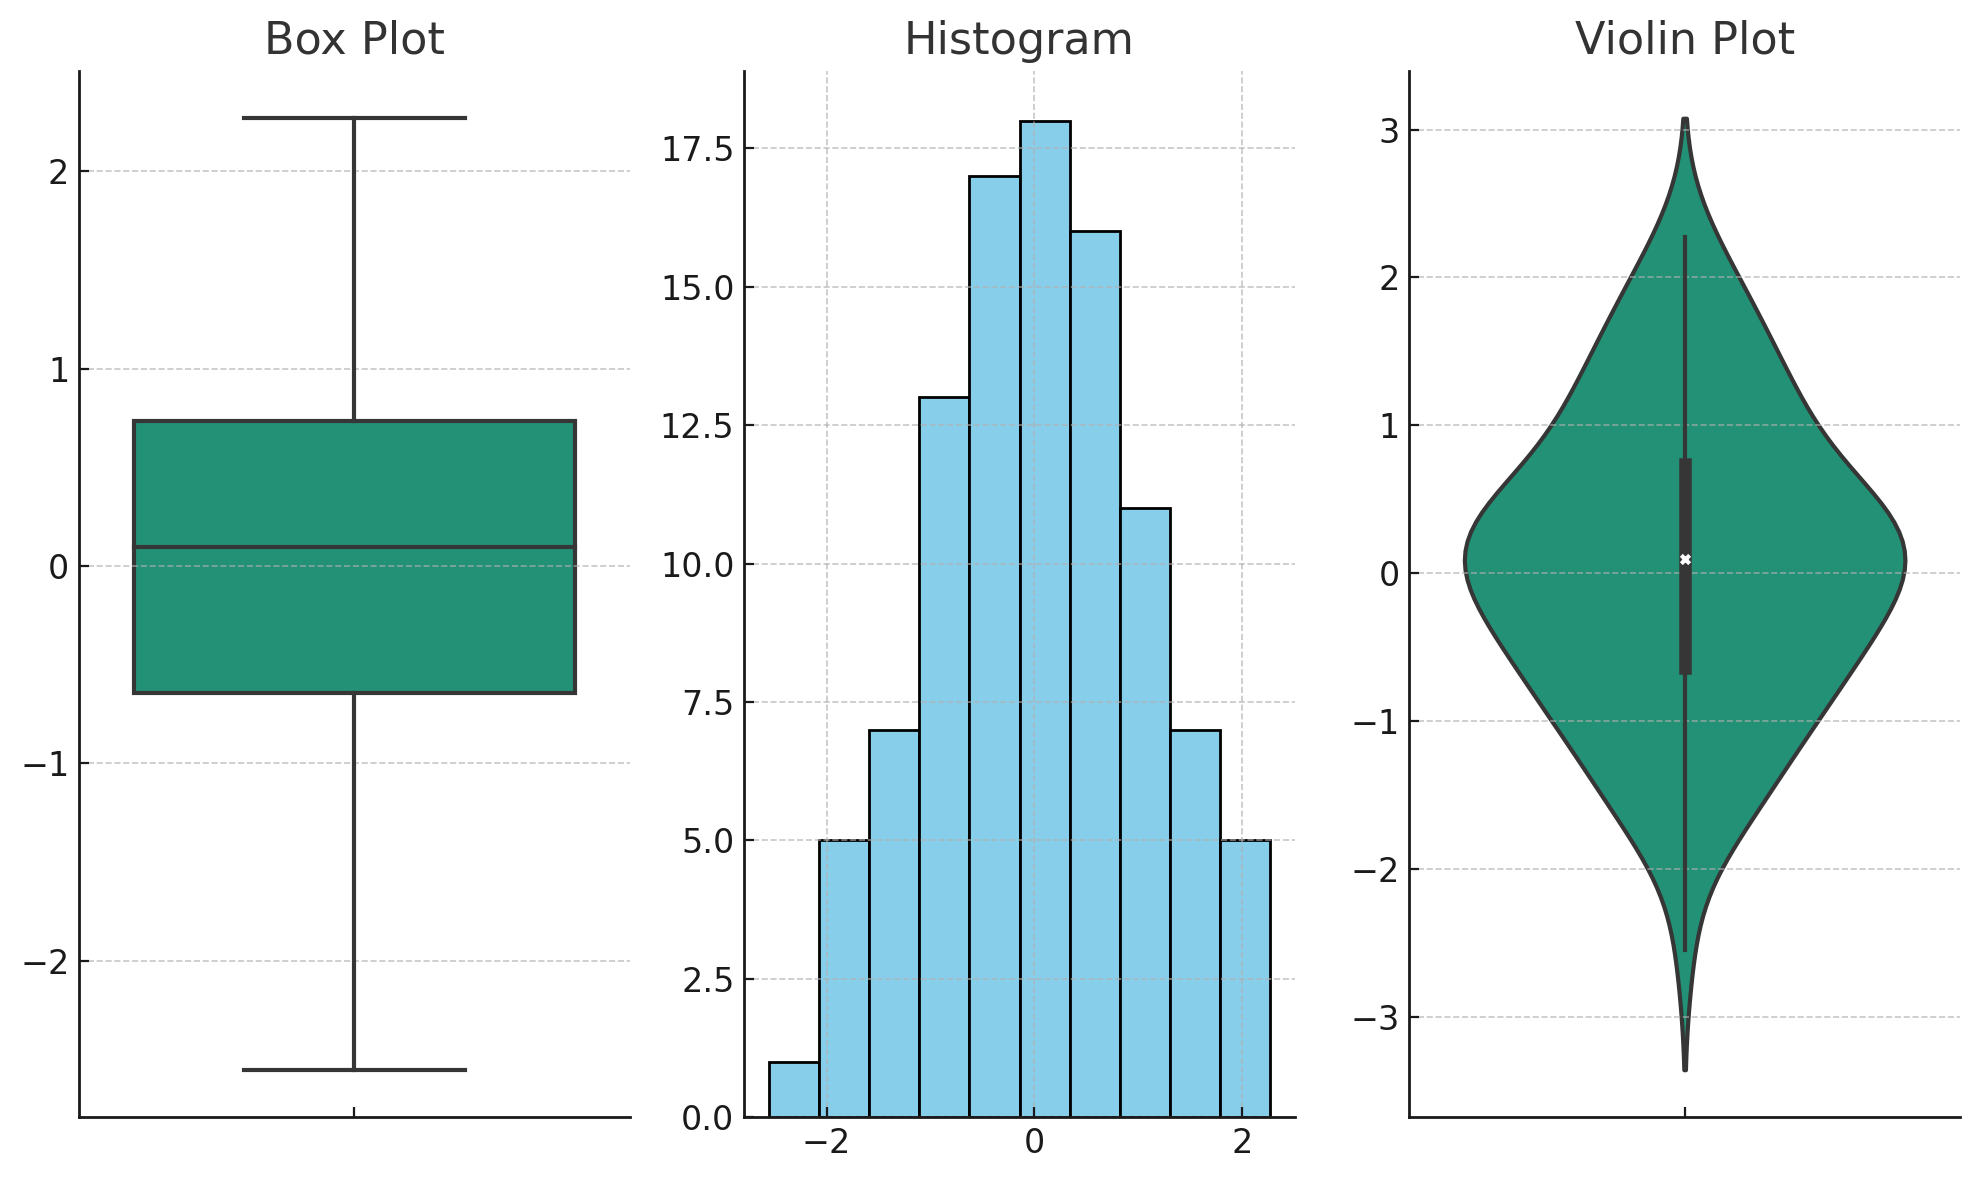
\includegraphics[scale=0.5]{Images/Plot Interpretation.png}
    \end{center}

    \begin{enumerate}
        \item \textbf{Box Plot}: A box plot (or box-and-whisker plot) provides a visual summary of the key aspects of a distribution:
        \begin{itemize}
            \item \textbf{Central line}: Represents the median of the data. In our box plot, the median is around 0, indicating the central tendency of the distribution.
            \item \textbf{Box}: The edges of the box (the interquartile range, IQR) show the 25th percentile (Q1) and the 75th percentile (Q3) of the data. The length of the box indicates the spread 
            of the central 50\% of the data. A shorter box suggests less variability in the middle half of the data.
            \item \textbf{Whiskers}: Extend from the box to show the range of the data. Typically, they extend to 1.5 * IQR beyond the quartiles, though this can vary. Points beyond the whiskers are 
            considered outliers and are often plotted as individual points.
            \item \textbf{Outliers}: Points outside the whiskers are plotted individually, indicating that they are unusual compared to the rest of the data. In our plot, there are a few outliers on 
            both sides, indicating data points significantly higher or lower than the majority.
        \end{itemize}
        \item \textbf{Histogram}: A histogram displays the distribution of data by forming bins along the range of the data and then drawing bars to show the number of observations that fall in each bin:
        \begin{itemize}
            \item \textbf{Bins}: The x-axis represents bins or intervals of values. In our histogram, data is divided into 10 bins.
            \item \textbf{Height of bars}: The y-axis represents the frequency of data points within each bin. The height of a bar shows how many data points fall into that range.
            \item \textbf{Distribution shape}: The histogram helps identify the distribution shape of the data, whether it's normal, skewed, or bimodal, for example. Our histogram suggests a roughly 
            normal distribution, as the bars form a bell-shaped curve around the center.
        \end{itemize}
        \item \textbf{Violin Plot}: A violin plot combines elements of box plots and density plots, providing a deeper understanding of the distribution:
        \begin{itemize}
            \item \textbf{Outer shape}: Represents the kernel density estimation of the data, showing the distribution's density. Thicker sections of the violin plot indicate a higher density of data 
            points, while thinner sections indicate lower density.
            \item \textbf{Inner box plot}: Often included within the violin, showing the median (central dot) and the interquartile range (thick bar). The violin plot in our example shows a median 
            around 0, similar to the box plot, with the bulk of data points concentrated around the center, indicating the central tendency and variability.
            \item \textbf{Width}: The width of the violin at different values indicates the density of the data at those values. In our plot, the widest part is around the median, suggesting the highest 
            density of data points is near the center of the distribution.
        \end{itemize}
    \end{enumerate}

    \subsubsection*{IQR}

    The Interquartile Range (IQR) is a measure of statistical dispersion, or variability, that indicates the spread of the middle 50\% of a dataset. It's calculated as the difference between the 75th 
    percentile (Q3) and the 25th percentile (Q1) of the data. The IQR is used to build box plots, as we've seen, and is helpful for identifying outliers.

    In essence, the IQR can be calculated with

    \begin{center}
        \begin{highlightbox}
            \text{IQR} = Q3 - Q1.
        \end{highlightbox}
    \end{center}
    where
    \begin{itemize}
        \item $Q1$ (the first quartile) is the median of the first half of the dataset (the 25th percentile).
        \item $Q3$ (the third quartile) is the median of the second half of the dataset (the 75th percentile).
    \end{itemize}

    \begin{highlight}[IQR Strategy]
        The steps to calculate the IQR are as follows:
        \begin{enumerate}
            \item \textbf{Order the Data}: Arrange the data points in ascending order.
            \item \textbf{Find the Median (Q2)}: This divides the dataset into two halves.
            \item \textbf{Find Q1 and Q3}:
            \begin{itemize}
                \item $Q1$ is the median of the data points to the left of the median of the dataset.
                \item $Q3$ is the median of the data points to the right of the median.
            \end{itemize}
            \item \textbf{Calculate the IQR}: Subtract $Q1$ from $Q3$.
        \end{enumerate}
    \end{highlight}

    IQR is important because:
    \begin{itemize}
        \item \textbf{Resistant to Outliers}: Unlike range and standard deviation, the IQR focuses on the middle bulk of the data and is not affected by outliers. This makes it a more robust measure 
        of spread for skewed distributions.
        \item \textbf{Identifying Outliers}: The IQR is used to define outliers. A common rule is that an outlier is any data point that lies more than 1.5 times the IQR above the third quartile (Q3) 
        or below the first quartile (Q1).
    \end{itemize}

    \begin{highlight}[IQR Example]
        Consider the sample data set \texttt{3,7,5,8,6,9}:

        \begin{enumerate}
            \item \textbf{Ordered Data Set}: \texttt{3,5,6,7,8,9}
            \item \textbf{Median}: The median of this data set is $\frac{6 + 7}{2} = 6.5$
            \item \textbf{Find Q1 and Q3}:
            \begin{itemize}
                \item $Q1$ is the median of the lower 50\%, \texttt{(3,5,6)}, and is 5
                \item $Q3$ is the median of the upper 50\%, \texttt{(7,8,9)}, and is 8
            \end{itemize}
            \item \textbf{Calculate IQR} $IQR = Q3 - Q1 = 8 - 5 = 3$
        \end{enumerate}
    \end{highlight}

    \subsubsection*{Skew}

    Skewness is a measure of the asymmetry of the probability distribution of a real-valued random variable. In simpler terms, it's a way to describe the direction and extent to which a distribution 
    deviates from a normal distribution, where the mean, median, and mode are all the same.

    The different types of skews are:

    \begin{itemize}
        \item \textbf{Positive Skew (Right-Skewed)}: The tail on the right side of the distribution is longer or fatter than the left side. In a positively skewed distribution, the mean is typically 
        greater than the median, which is greater than the mode. This type of skew indicates that there are a number of exceptionally high values pulling the mean to the right.
        \item \textbf{Negative Skew (Left-Skewed)}: The tail on the left side of the distribution is longer or fatter than the right side. In a negatively skewed distribution, the mean is typically 
        less than the median, which is less than the mode. This skew indicates that there are a number of exceptionally low values pulling the mean to the left.
    \end{itemize}

    When interpreting the central tendency from a skewed data set, the mean is located on the side of the skew. We can see the different central tendencies of each type of skew below.

    \begin{center}
        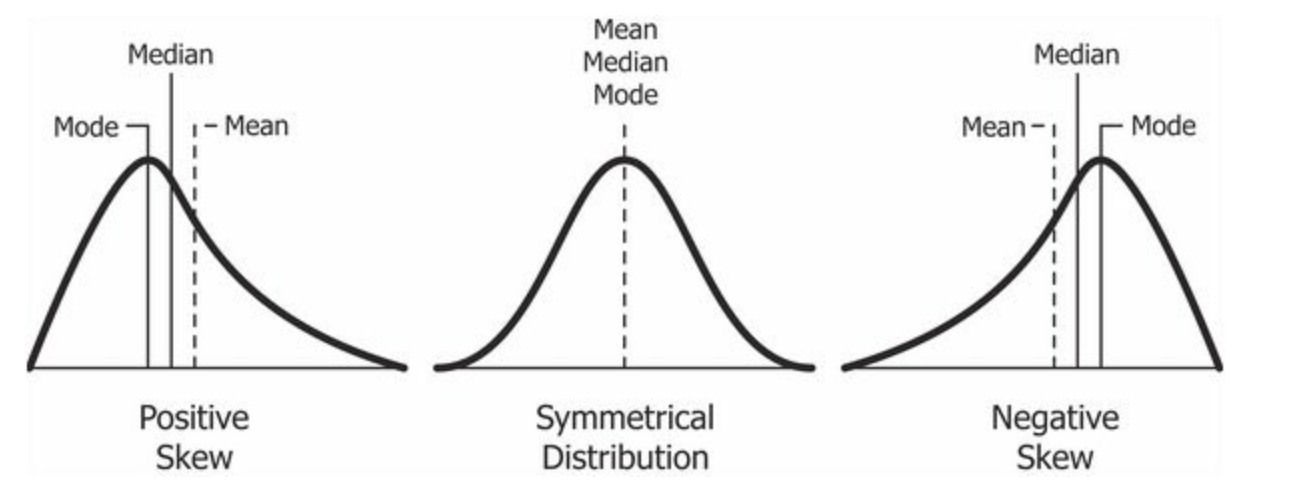
\includegraphics[scale = 0.75]{Images/Skew.png}
    \end{center}

    \subsubsection*{Probability}

    In probability, particularly sets, there is certain terminology that is used. In the context of set notation, the following are terms that are pertinent to probability theory are

    \begin{enumerate}
        \item \textbf{Complement}: The complement of a set $A$, denoted as $A'$ or $A^{c}$, represents all elements not in $A$ but within the universal set $U$, which contains all possible outcomes. 
        In probability, the complement of an event represents the probability that the event does not happen.
        \begin{itemize}
            \item \textbf{Notation}: $A^{c}$ of $A'$
            \item \textbf{Formula}: The formula for calculating the complement of the probability of $A$ $(P(A))$ is
            \begin{center}
                \begin{highlightbox}
                    P(A') = 1 - P(A)
                \end{highlightbox}
            \end{center}
        \end{itemize}
        \item \textbf{Intersection}: The intersection of two sets $A$ and $B$, denoted as $A \cap B$, represents all elements that are both in $A$ and in $B$. In probability, the intersection of two
        events represents the probability that both events occur simultaneously.
        \begin{itemize}
            \item \textbf{Notation}: $A \cap B$
            \item \textbf{Formula}: The formula for calculating $P(A \cap B)$ depends on whether events $A$ and $B$ are independent or dependent.
            \begin{itemize}
                \item For \textbf{independent events}
                \begin{center}
                    \begin{highlightbox}
                        P(A \cap B) = P(A) \cdot P(B)
                    \end{highlightbox}
                \end{center}
                \item For \textbf{dependent events}, you need additional information to calculate $P(A \cap B)$ directly.
            \end{itemize}
        \end{itemize}
        \item \textbf{Union} The union of two sets $A$ and $B$, denoted as $A \cup B$, represents all elements that are in $A$, in $B$, or in both. In probability, the union of two events represents 
        the probability that at least one of the events occurs.
        \begin{itemize}
            \item \textbf{Notation}: $A \cup B$
            \item \textbf{Formula}: The formula for calculating the union of two probabilities is
            \begin{center}
                \begin{highlightbox}
                    P(A \cup B) = P(A) + P(B) - P(A \cap B)
                \end{highlightbox}
            \end{center}
        \end{itemize}
    \end{enumerate}

    \subsubsection*{Event Space}

    Event Space, also known as Sample Space in the context of probability, is a fundamental concept that represents all possible outcomes of a probabilistic experiment. Understanding the event space 
    is crucial for calculating probabilities, as it sets the stage for identifying specific events within the realm of all outcomes.

    We define event and sample space as the following:
    \begin{itemize}
        \item \textbf{Sample Space (S)}: The set of all possible outcomes of a probabilistic experiment. It could be finite or infinite, depending on the nature of the experiment.
        \item \textbf{Event (E)}: Any subset of the sample space. An event is a specific outcome or a combination of outcomes that we're interested in.
    \end{itemize}

    The type of sample spaces are the following:
    \begin{itemize}
        \item \textbf{Finite Sample Space}: When the number of possible outcomes is countable and limited. For example, rolling a six-sided die has a finite sample space of \texttt{\{1, 2, 3, 4, 5, 6\}}.
        \item \textbf{Infinite Sample Space}: When the number of possible outcomes is uncountable or unlimited. For example, measuring the time it takes for something to happen could have an infinite 
        number of possible outcomes.
    \end{itemize}

    \subsubsection*{Conditional Probability}

    Conditional probability is a fundamental concept in probability theory that deals with finding the probability of an event given that another event has occurred. This concept is crucial for 
    understanding the relationship between two events and how the occurrence of one event affects the likelihood of another.

    The conditional probability of an event $A$ given that event $B$ has occurred is denoted as $P(A|B)$ and is defined as:

    \begin{center}
        \begin{highlightbox}
            P(A|B) = \frac{P(A \cap B)}{P(B)}
        \end{highlightbox}
    \end{center}
    provided that $P(B) > 0$.

    The way we can interpret conditional probability is the following:
    \begin{itemize}
        \item $P(A|B)$ is read as `the probability of $A$ given $B$'.
        \item It quantifies how the probability of $A$ changes when we know that $B$ has occurred.
        \item This is different from the probability of $A$ occurring in isolation, without any knowledge about $B$.
    \end{itemize}
    Key points that can be taken away from conditional probability:
    \begin{itemize}
        \item \textbf{Dependence}: Conditional probability is used when the occurrence of one event affects the probability of another, indicating a dependency between events.
        \item \textbf{Recalculation of Probabilities}: Knowing that $B$ has occurred may change the sample space and, consequently, the probabilities of subsequent events.
        \item \textbf{Bayes' Theorem}: A fundamental result that follows from the concept of conditional probability, allowing for the update of probabilities as more evidence becomes available.
    \end{itemize}

    \subsubsection*{Bayes Theorem}

    Bayes' Theorem is a powerful tool in probability theory that allows us to update our beliefs about the probability of an event based on new evidence. It's named after Thomas Bayes (1701-1761), a 
    British statistician and philosopher. This theorem is particularly useful in the field of data science for making predictions under uncertainty and has applications ranging from spam filtering 
    to medical diagnosis.

    Bayes' Theorem is as follows:
    \begin{center}
        \begin{highlightbox}
            P(A|B) = \frac{P(B|A) \cdot P(A)}{P(B)}
        \end{highlightbox}
    \end{center}
    where:
    \begin{itemize}
        \item $P(A|B)$ is the posterior probability of event $A$ occurring given that $B$ has occurred.
        \item $P(B|A)$ is the likelihood, the probability of event $B$ occurring given that $A$ has occurred.
        \item $P(A)$ is the prior probability of event $A$ occurring.
        \item $P(B)$ is the marginal probability of event $B$ occurring.
    \end{itemize}

    \subsubsection*{Independence}

    Independence is a key concept in probability theory that describes a situation where the occurrence of one event does not affect the probability of another event occurring. Two events, $A$ and $B$,
    considered independent if and only if the occurrence of $A$ has no impact on the probability of $B$ happening, and vice versa.

    The formal definition of independence is two events $A$ and $B$ are independent if any of the following equivalent statements holds true:
    \begin{enumerate}
        \item The probability that both $A$ and $B$ occur is equal to the product of the probabilities of each event occurring separately:
        \begin{equation*}
            P(A \cap B) = P(A) \cdot P(B)
        \end{equation*}
        \item The conditional probability of $A$ given $B$ is the same as the probability of $A$, and vice versa:
        \begin{align*}
            P(A|B) & = P(A) \\
            P(B|A) & = P(B)
        \end{align*}
    \end{enumerate}
    Independence intuitively means that knowing whether $B$ shas occurred provides no information about the occurrence of $A$, and the reverse is also true. For instance, if you flip a fair coin twice,
    the outcome of the first flip does not influence the outcome of the second flip; these events are independent.
\end{examnotes}

\begin{cheatsheet}{Exam 1 Cheat Sheet}
    \subsubsection*{The Rule of Sum}

    If there are $A$ ways to do something and $B$ ways to do another thing, and these two things cannot happen at the same time, then there are $A + B$ ways to choose one of these actions.

    \subsubsection*{The Rule of Product}

    If there are $A$ ways to do something and $B$ ways to do another thing after that, then there are $A \cdot B$ ways to perform both actions.

    \subsubsection*{Permutations}

    Permutations are the arrangements of objects in a specific order. For arranging $r$ objects out of $n$ available objects, the formula is

    \begin{equation*}
        ^{n}P_{r} = \frac{n!}{(n - r)!}
    \end{equation*}

    \subsubsection*{Combinations}

    Combinations refer to the selection of objects without regard to the order. The number of ways to choose r objects from n different objects is given by

    \begin{equation*}
        {n \choose r} = \frac{n!}{r!(n - r)!}
    \end{equation*}

    \subsubsection*{Binomial Theorem}

    Provides a formula for the expansion of powers of a binomial (sum of two terms).

    \begin{equation*}
        (a + b)^{n} = \sum_{k = 0}^{n} {n \choose k} \cdot a^{n - k} \cdot b^{k}
    \end{equation*}

    \subsubsection*{Binomial Distribution}

    A binomial distribution is a discrete probability distribution that models the number of successes in a fixed number of independent Bernoulli trials

    \begin{equation*}
        P(x = k) = {n \choose k} \cdot p^{k} \cdot (1 - p)^{n - k}
    \end{equation*}
    \begin{itemize}
        \item $\binom{n}{k}$ (read as `$n$ choose $k$') is the binomial coefficient, representing the number of ways to choose $k$ successes from $n$ trials.
        \item $p$ is the probability of success on an individual trial.
        \item $1 - p$ is the probability of failure (since the trials are binary, the sum of the probabilities of success and failure is 1).
        \item $p^{k}$ is the probability of having $k$ successes.
        \item $(1 - p)^{n - k}$ is the probability of having $n - k$ failures.
    \end{itemize}

    \subsubsection*{IQR}

    The spread of the middle 50\% of the data set

    \begin{equation*}
        \text{IQR} = Q3 - Q1
    \end{equation*}

    \subsubsection*{Skew}

    \begin{itemize}
        \item \textbf{Positive Skew (Right-Skewed)}: The tail on the right side of the distribution is longer or fatter than the left side. In a positively skewed distribution, the mean is typically 
        greater than the median, which is greater than the mode. This type of skew indicates that there are a number of exceptionally high values pulling the mean to the right.
        \item \textbf{Negative Skew (Left-Skewed)}: The tail on the left side of the distribution is longer or fatter than the right side. In a negatively skewed distribution, the mean is typically 
        less than the median, which is less than the mode. This skew indicates that there are a number of exceptionally low values pulling the mean to the left.
    \end{itemize}

    \subsubsection*{Complement}

    \begin{equation*}
        P(A') = 1 - P(A)
    \end{equation*}

    \subsubsection*{Intersection}

    For \textbf{independent events}, the intersection is

    \begin{equation*}
        P(A \cap B) = P(A) \cdot P(B)
    \end{equation*}

    \subsubsection*{Union}

    The union of two probabilistic events are

    \begin{equation*}
        P(A \cup B) = P(A) + P(B) - P(A \cap B)
    \end{equation*}

    \subsubsection*{Conditional Probability}

    The conditional probability of an event $A$ given that event $B$ has occurred is denoted as $P(A|B)$ and is defined as

    \begin{equation*}
        P(A|B) = \frac{P(A \cap B)}{P(B)}
    \end{equation*}

    \subsubsection*{Bayes Theorem}

    \begin{equation*}
        P(A|B) = \frac{P(B|A) \cdot P(A)}{P(B)}
    \end{equation*}
    \begin{itemize}
        \item $P(A|B)$ is the posterior probability of event $A$ occurring given that $B$ has occurred.
        \item $P(B|A)$ is the likelihood, the probability of event $B$ occurring given that $A$ has occurred.
        \item $P(A)$ is the prior probability of event $A$ occurring.
        \item $P(B)$ is the marginal probability of event $B$ occurring.
    \end{itemize}

    \subsubsection*{Independence}
    The formal definition of independence is two events $A$ and $B$ are independent if any of the following equivalent statements holds true:
    \begin{itemize}
        \item The probability that both $A$ and $B$ occur is equal to the product of the probabilities of each event occurring separately:
        \begin{equation*}
            P(A \cap B) = P(A) \cdot P(B)
        \end{equation*}
        \item The conditional probability of $A$ given $B$ is the same as the probability of $A$, and vice versa:
        \begin{align*}
            P(A|B) & = P(A) \\
            P(B|A) & = P(B)
        \end{align*}
    \end{itemize}
\end{cheatsheet}